% \chapter{少资源微调——开源工具包构建}

% \section{参数高效微调代码框架}

% \subsection{动机}

% 在本节中,首先介绍微调的统一公式。随后,强调微调的一系列关键特性,重点关注实现方面,这凸显了对新型工具包的迫切需求,以支持微调方法的研究和发展。


% \subsubsection{微调的统一公式}

% 尽管微调原则上不仅限于特定类型的神经网络,但目前几乎所有微调方法都应用于基于Transformers架构的预训练模型~\cite{devlin2018bert, liu2019roberta, raffel2019exploring, brown2020language}。一个由$\Theta$参数化的预训练模型$\mathcal{M}$由多个子模块$m$组成,其中隐藏表示$\mathbf{h}$通过子模块传递以生成新的隐藏表示$\mathbf{h}'$,即$\mathbf{h}' = m(\mathbf{h})$。

% \begin{figure*}[!htbp]
%     \centering
%     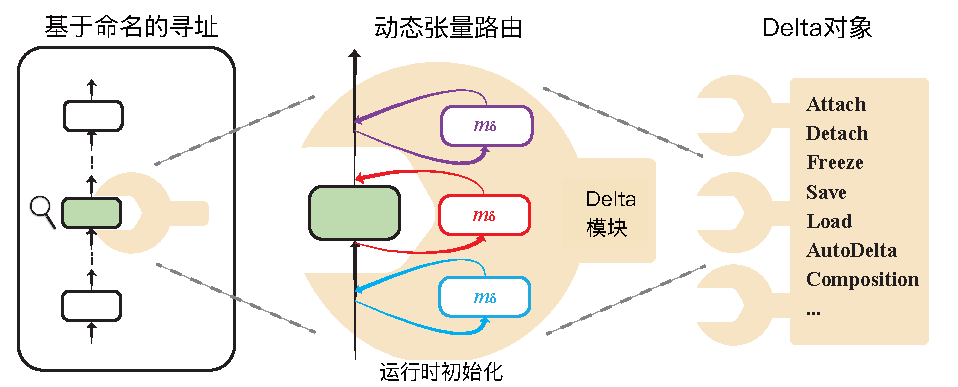
\includegraphics[width=0.9\linewidth]{odfigs/Framework.zh.pdf}
%     \caption{OpenDelta的整体框架}
%     \label{fig:framework}
% \end{figure*}

% 将预训练模型$\mathcal{M}$适应下游任务的过程是将原始参数$\Theta$更新为$\Theta'$。在全参数微调中,所有参数都可以更新,即$|\Delta \Theta| = |\Theta|$。相比之下,微调仅更新一小部分参数,即$|\Delta \Theta| \ll |\Theta|$。

% 尽管微调方法在具体形式上存在显著差异,~\citet{he2022unified}将它们统一为对隐藏表示$\mathbf{h}$的修改$\Delta \mathbf{h}$的特殊形式。$\Delta \mathbf{h}$通过将隐藏状态$\mathbf{h}_{{\delta}}$传递给\textit{delta模块} $m_\delta$生成。形式上,
% \begin{equation}
% \label{equ:unifydelta}
% \mathbf{h} \leftarrow \mathbf{h} + \Delta \mathbf{h} = \mathbf{h} + m_\delta(\mathbf{h}_{{\delta}}),
% \end{equation}
% 其中$\leftarrow$表示替换原始的$\mathbf{h}$,$\mathbf{h}_{{\delta}}$可以与$\mathbf{h}$相同或不同。


% \subsubsection{微调的关键特性}

% 从公式(\ref{equ:unifydelta})中可以看出微调方法的几个关键特性。

% \textbf{张量重定向。} 微调的第一个特性是能够重定向隐藏状态的流动。在预训练模型中,隐藏状态的流动形成一个静态图,隐藏状态作为节点,子模块作为边上的变换。如公式(\ref{equ:unifydelta})所示,引入边变换$m_\delta$将节点$\mathbf{h}_{\delta}$重定向并注入到另一个节点$\mathbf{h}$中,创建了原始模型架构中不存在的新隐藏状态流动。OpenDelta的实现应能够在无需硬编码的情况下实现这种张量重定向。

% \textbf{灵活性。}
% 公式(\ref{equ:unifydelta})允许输入隐藏状态和输出隐藏状态位于主干模型$\mathcal{M}$中的任何位置。例如,AdapterDrop~\cite{ruckle-etal-2021-adapterdrop}观察到,仅将delta模块应用于Transformer层的上半部分比应用于下半部分效果更好。应用位置的灵活性为探索delta模块的潜在结构提供了显著的机会~\cite{hu2022sparse}。然而,这也对实现提出了挑战,要求在实践中能够达到与理论框架相匹配的灵活性。

% \textbf{组合性。} 不同的微调方法可以共存,甚至可以在同一主干模型中组合使用~\cite{hu2022sparse},从而可能提升性能或支持多任务学习~\cite{pfeiffer2020adapterfusion}。因此,实现每个微调方法的独立性和易用性,同时允许多个模块的灵活组合至关重要。

% \textbf{动态性。} 在微调中,主干预训练模型通常作为多个任务的中心模型。为了服务于特定任务,delta模块被附加到主干模型上,创建任务特定的专家。当delta模块被移除时,主干模型恢复其作为通用语言模型的原始功能。这种基于微调的任务适应的动态性应被纳入OpenDelta中。


% \subsection{OpenDelta}

% 鉴于上述微调的关键特性,本文提出了OpenDelta。首先将介绍OpenDelta的概述,随后深入探讨该框架的关键实现。


% \begin{table*}
% \centering
% \caption{各参数高效微调方法在三种路由下的划分}
% \resizebox{\textwidth}{!}{
% \begin{tabular}{c|cccc}
% \toprule
% 方法 & 公式 & 默认位置 & 路径 & 运行时初始化  \\
% \midrule
% LoRA & $ m_\delta(\mathbf{h}_{\text{in}}) = \mathbf{h}_{\text{in}} \mathbf{A}\mathbf{B}$ & Query, Value & 公式(\ref{equ:para}) & 否  \\
% Adapter & $ m_\delta(\mathbf{h}_{\text{out}}) = \sigma(\mathbf{h}_{\text{out}} \mathbf{W}_1)\mathbf{W}_2$ &{ATTN, FFN}  & { 公式(\ref{equ:after}) } & {是}  \\
% Bitfit & $ m_\delta(\mathbf{h}_{\text{out}}) = \mathbf{b}$& ATTN, FFN, LayerNorm & 公式(\ref{equ:after}) & 否 \\
% Prefix Tuning & $ m_\delta(\mathbf{h}_{\text{out}}) = [\text{MLP}(\mathbf{p}); \mathbf{h}_{\text{out}}]$  & Key, Value & 公式(\ref{equ:after})  & 是 \\
% \bottomrule
% \end{tabular}
% }
% \label{tab:defaultconfig} 
% \end{table*}

% \subsubsection{框架}

% 要进行微调,需要两个前提条件:一个预训练语言模型$\mathcal{M}$和所谓“\textit{修改模块}”,即用户指定的子模块$m_i$列表,delta模块应该应用于这些子模块。目标是构建一个\textit{delta对象}。delta对象是一组delta模块的集合,通常位于$\mathcal{M}$中的不同位置,作为一个整体来使预训练模型适应下游任务。构建delta对象分为三个步骤:
% 首先,使用\textit{基于名称的寻址}获取修改模块的指针。其次,构建一个包含未初始化delta模块的delta对象。
% 第三,使用\textit{动态张量重定向}技术将修改模块中的张量路径修改为delta模块中的路径。

% 在隐藏状态的更新路径建立后,执行\textit{运行时初始化}以初始化delta对象。
% 在delta对象构建完成后,将其附加到主干模型上。随后,提供一个简单的功能接口,以关闭主干模型中的梯度计算,仅计算delta对象中的参数梯度。
% 训练完成后,提供一个简单的接口用于仅保存delta对象,这显著减少了主干模型的存储需求。

% OpenDelta的整体框架如图~\ref{fig:framework}所示。接下来,将介绍支持构建delta对象的关键实现。


% \begin{figure}
%     \centering
%     \begin{minipage}{0.96\textwidth}
%     \begin{lstlisting}[language=Python]
%     model = AutoModel.from_pretrained("bert-base-cased")
    
%     + from bigmodelvis import Visualization
%     + Visualization(model).structure_graph()
%     + from opendelta import LoraModel
%     + delta_model = LoraModel(backbone_model=model, modified_modules=["output.dense", "query"])
%     + delta_model.freeze_module(exclude=["deltas", "pooler"], set_state_dict=True)
%     + Visualization(model).structure_graph()
    
%     trainer.train()
%     \end{lstlisting}
%     \end{minipage} 
%     \caption{OpenDelta 的基本用法示例}
%     \label{fig:basic_usage} 
% \end{figure}


% \subsubsection{关键实现}
% 上述框架通过四个关键实现来完成,即基于名称的寻址、动态张量重路由、运行时初始化和可视化系统。

% 该参数高效微调框架为大型预训练模型提供了一套全面的轻量级调整解决方案,通过精心设计的架构实现高度灵活而简便的模型适配。该系统遵循三阶段工作流程:首先通过智能定位算法获取目标子模块的指针,然后构建包含未初始化调优组件的结构化对象,最后应用张量流重定向技术将原始计算路径修改为包含调优组件的新路径。

% 该框架的技术核心由四大关键组件构成。首先,智能模块定位机制支持多种匹配模式,包括层次模式简化、尾部特征匹配和高级模式表达式,大幅简化了用户指定目标位置的复杂度。其次,计算流动态重构系统提供了三种不同的隐藏态传递方案,分别基于输入状态修改、输出状态修改和平行计算修改,足以支持主流调优方法的各种需求。第三,自适应维度感知技术通过伪输入传播自动检测并匹配隐藏状态的形状和维度,消除了手动检查模型代码的需求。最后,层级结构可视化工具利用Transformer架构的重复性特征,提供了清晰直观的参数与结构展示,方便用户验证调优组件的正确部署。

% 该框架的设计理念体现在三个突出特性中:使用便捷性、模块化设计和扩展灵活性。在便捷性方面,用户仅需添加少量代码即可从传统全参数微调迁移到参数高效微调,同时提供自动配置机制以支持不熟悉底层细节的实践者。在模块化设计上,框架允许调优组件的独立附加与分离操作,使单一主干模型能够通过动态切换不同调优组件来处理多样化任务,极大提高了模型的复用效率。在扩展性方面,框架建立了统一的命名规范与映射体系,能够无缝支持不同架构的预训练模型,并提供检查点加载功能以方便迁移学习应用。

% 总体而言,该框架通过精炼的接口设计和强大的底层实现,显著降低了参数高效微调的技术门槛,为研究人员和开发者提供了一个理想的大模型调优工具集,既满足了实验灵活性需求,又优化了计算资源利用效率,为大模型的广泛应用创造了有利条件。
% \textbf{基于名称的寻址。} 首先,需要获取应用了增量模块的目标子模块的指针。在实践中,可以通过使用子模块的名称有效地检索到该指针。由于子模块以树状结构组织,本文采用深度优先搜索来查找与提供名称匹配的子模块。此搜索会生成一个完整路径,该路径由从根到匹配子模块的所有名称组成,从而准确匹配子模块。

% 然而,直接编写子模块的完整路径可能不切实际,因此本文设计了几种简化方法,使寻址更简单且更易读~\footnote{\url{https://opendelta.readthedocs.io/en/latest/notes/namebasedaddr.html}}。其中一种简化方法是利用 Transformer 层的重复性,许多参数高效微调方法通过在每一层的相同类型子模块中添加增量模块来实现。例如,当用户指定 \texttt{attention} 时,他们可能希望在所有 Transformer 层的注意力子模块中应用增量模块。为了满足这一需求,本文提供了一种尾部匹配机制,可以根据子模块的名称自动匹配它们。对于更复杂的位置配置,本文允许基于正则表达式进行匹配,并使用自定义设计的 Web 界面进行基于 Web 的选择。

% \textbf{动态张量重路由。} OpenDelta 与其他实现的一个根本区别在于,它能够在不需要修改主干模块代码的情况下添加增量模块。这一特性需要通过增量模块动态重路由张量,并将其重新注入主干模型。

% 为了实现这一重路由,本文将子模块的原始前向函数包装在一个包装函数中,并用包装函数替换原始前向函数。为了确保无缝替换,本文使用装饰器继承原始函数的属性,包括输入/输出、文档字符串等。在包装函数中,本文实现了三种不同的隐藏状态路由,考虑了原子模块和增量模块的顺序。

% 第一种路由使用 $m_i$ 的输入隐藏状态 $\mathbf{h}_\text{in}$ 作为修改目标和增量模块的输入。将其通过增量模块得到输出 $m_\delta(\mathbf{h}_\text{in})$,并将其合并到 $\mathbf{h}_\text{in}$ 中。形式上:
% \begin{equation}
% \label{equ:in}
% \mathbf{h}_\text{in}\leftarrow\mathbf{h}_\text{in} + m_\delta(\mathbf{h}_\text{in}).
% \end{equation}

% 第二种路由使用 $m_i$ 的输出隐藏状态 $\mathbf{h}_\text{out}$ 作为修改目标:
% \begin{equation}
% \label{equ:after}
% \mathbf{h}_\text{out}\leftarrow\mathbf{h}_\text{out} + m_\delta(\mathbf{h}_\text{out}).
% \end{equation}

% 第三种路由利用输入隐藏状态 $\mathbf{h}_\text{in}$ 作为增量模块的输入,并将输出隐藏状态 $\mathbf{h}_\text{out}$ 设置为修改目标:
% \begin{equation}
% \label{equ:para}
% \mathbf{h}_{\text{out}}\leftarrow\mathbf{h}_\text{out} + m_\delta(\mathbf{h}_\text{in}).
% \end{equation}

% 虽然这三种路由并不一定涵盖增量模块与主干模型之间所有可能的关系,但它们足以支持大多数流行的参数高效微调方法。表~\ref{tab:defaultconfig} 中展示了各参数高效微调方法在这三种路由下的划分。默认位置指的是当未指定特定子模块时,delta模块附加的位置。$\mathbf{A}$,$\mathbf{B}$,$\mathbf{W}_1$,$\mathbf{W}_2$是权重矩阵,$\mathbf{b}$是偏置向量。MLP($\cdot$)是多层感知网络。$[\cdot;\cdot]$表示张量的拼接。$\sigma$是激活函数。运行时初始化显示OpenDelta的实现是否使用此技术。然而,本文仍对根据需要引入更多路由持开放态度。

% \textbf{运行时初始化。} 为了确保增量模块中的权重矩阵在形状和维度上与隐藏状态匹配,必须考虑模型配置中未指定形状的隐藏状态。在传统实现中,这需要手动检查主干模型的代码。然而,OpenDelta 通过将伪输入传递到主干模型中来自动化这一过程,从而在隐藏状态从输入传播到输出时自动确定其形状。


% \textbf{可视化系统。} 由于参数高效微调提供了灵活性和动态性,因此通过验证增量模块是否按指定添加来确保增量对象的正确构建至关重要。然而,直接打印大型预训练模型会导致输出内容过于庞大。

% 为了解决这一问题,本文提供了一个可视化系统,该系统利用 Transformer 架构中的重复性。具体来说,本文将重复的层折叠起来,并清晰地打印参数信息。通过将增量模块添加到主干模型中,用户可以轻松地通过可视化观察到模型中的变化。可视化的示例如图~\ref{fig:after_lora} 所示。由于可视化系统在参数高效微调之外的场景中也很有用,因此它已被分离为一个独立的包,名为“\texttt{bigmodelvis}”~\footnote{\url{https://pypi.org/project/bigmodelvis/}}。

% \begin{figure}
%     \centering
%     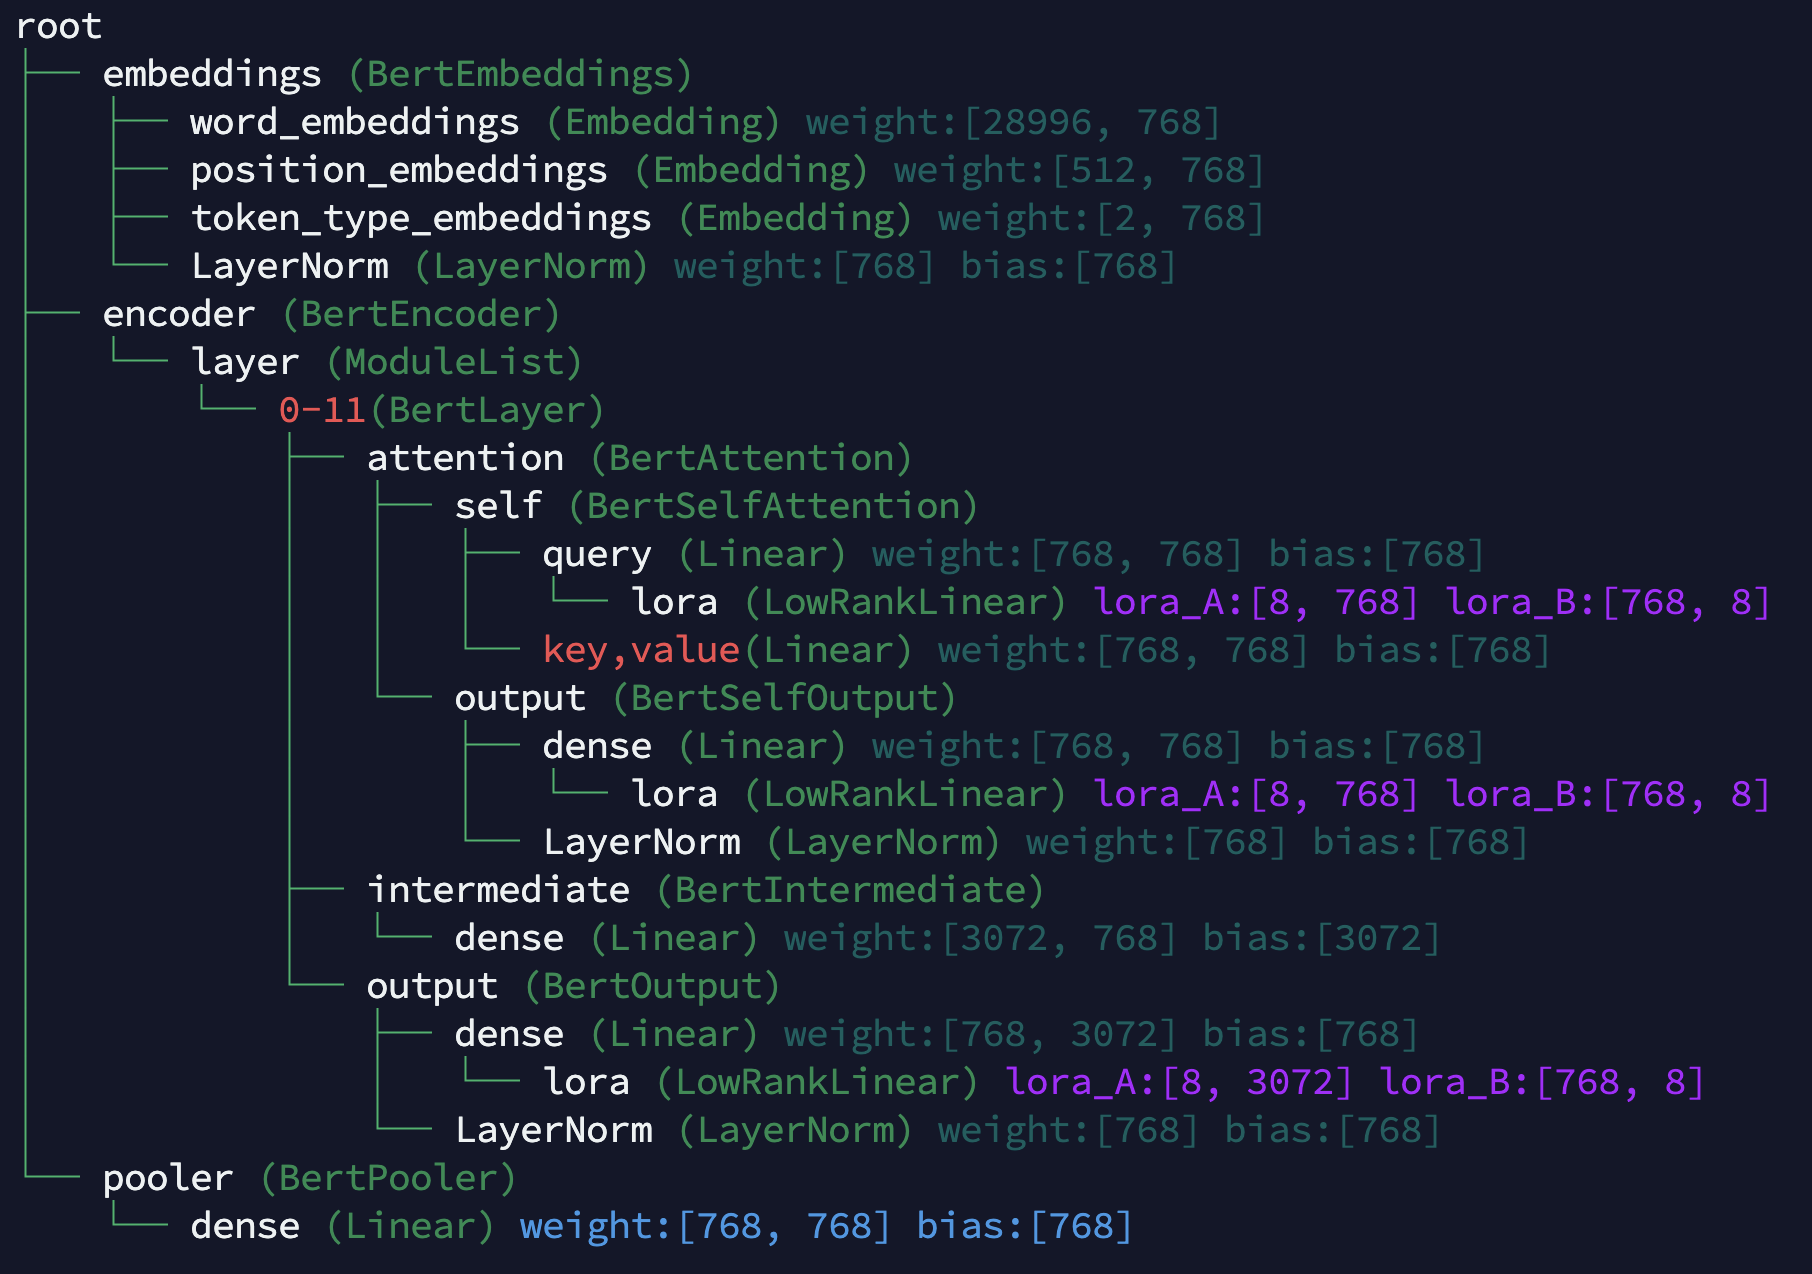
\includegraphics[width=\linewidth]{odfigs/bert_with_lora.png}
%     \caption{附加 LoRA 模块后主干模型状态的可视化}
%     \label{fig:after_lora}
% \end{figure}

% \subsection{案例与特性}
% 在本节中,本文提供了 OpenDelta 的使用案例,展示了 OpenDelta 的三个特性,即简洁性、模块化和可扩展性。

% \begin{figure}[hbt!]
% \centering
% \begin{minipage}{0.94\textwidth}
% \begin{lstlisting}[language=Python]
% def multi_task(delta_model, input_text):
%     global model # 跨任务使用相同的主干模型。
%     delta_model.attach()
%     print(tokenizer.decode(model.generate(input_ids=tokenize(input_text))))
%     delta_model.detach()
% multi_task("What the commmon career of Newton ad einstein?", spelling_delta)
% # >>> "What was the common career of Newton and Einstein?"
% multi_task("What was the common career of Newton and Einstein?", topic_delta)
% # >>> "The question's topic is science."
% multi_task("What was the common career of Newton and Einstein?", question_delta)
% # >>> "Physicists."
% \end{lstlisting}
% \end{minipage} 
% \caption{通过 OpenDelta 进行多任务学习}
% \label{fig:code_multi_task} 
% \end{figure}

% \subsubsection{简洁性}

% \textbf{从微调迁移。} 为了便于从现有的全参数微调迁移到参数高效微调,只需修改几行代码,如图~\ref{fig:basic_usage} 所示。`+' 符号表示启用 delta 微调所需的额外代码。如果用户对主干模型熟悉,可视化部分是可选的。最初,在传统的全参数微调中,预训练模型从外部库(如 Huggingface Transformers)加载(第 1 行),并训练模型(第 10 行)。为了引入参数高效微调,添加并执行第 3-8 行。首先,可以选择可视化主干模型以确定目标 ``\texttt{modified\_modules}''。然后,创建一个增量对象(如 LoRA)并将其附加到主干模型。接着,冻结除增量模块和随机初始化的分类头之外的模型参数。``\texttt{set\_state\_dict=True}'' 参数用于从模型检查点中移除不可训练的参数。最后,可视化主干模型的子模块以验证增量模块的成功创建和附加。可视化结果的示例如图~\ref{fig:after_lora} 所示。

% \textbf{AutoDelta 机制。} OpenDelta 的实现支持高度复杂的增量模块设计,以满足多样化的实验需求。然而,对于可能不熟悉参数高效微调机制的实践者,提供一个默认的增量模块配置是很有必要的。
% 尽管各种主干模型共享 Transformer 架构,但它们的子模块命名规范差异很大。为了解决这个问题,本文建立了一个通用的命名规范,并使用映射技术将模型特定的命名规范映射到通用规范~\footnote{\url{https://opendelta.readthedocs.io/en/latest/notes/unifyname.html}}。这使得 AutoDelta 机制能够无缝支持。
% 图~\ref{fig:autodelta} 展示了,一旦指定了参数高效微调方法的类型,增量模块将以默认位置和适当的超参数附加到主干模型。本文在表~\ref{tab:defaultconfig} 中列出了每种参数高效微调方法的默认配置。此外,AutoDelta 机制还支持加载增量模块的微调检查点,而无需明确了解增量模块的类型和超参数。

% \begin{figure}[hbt!]
% \centering
% \begin{minipage}{0.94\linewidth}
% \begin{lstlisting}[language=Python]
% from opendelta import AutoDeltaModel, AutoDeltaConfig
% # 使用默认配置构建一个新的增量模块。
% delta_config = AutoDeltaConfig.from_dict({"delta_type":"lora"})
% delta_model = AutoDeltaModel.from_config(delta_config, backbone_model)
% # 加载增量模块的检查点。
% delta = AutoDeltaModel.from_finetuned("save_dir", backbone_model)
% \end{lstlisting}
% \end{minipage}
% \caption{使用 AutoDelta 机制的示例}
% \label{fig:autodelta}
% \end{figure}

% \subsubsection{模块化}
% OpenDelta 的第二个显著特性是模块化。它允许将每个增量对象独立地附加到主干模型或从主干模型中分离,从而为使用单一主干模型进行多任务处理提供了可能性。具体来说,假设与各种任务相关的数据依次呈现,其中每个数据触发将相应的增量对象附加到主干模型以进行处理,完成后增量对象被分离。图~\ref{fig:code_multi_task} 展示了一个说明此功能的案例,其中使用单一主干模型依次处理了三个任务。

\section{本章小结}
本文首先提出了稀疏结构搜索方法(S3Delta),该方法在多种DT模块混合的统一搜索空间中,通过显式稀疏控制进行可微分的DT结构搜索。实验证明了S3Delta在寻找最优DT模块结构方面的有效性,并推动了可训练参数减少的极限。其次,本文在构建的统一搜索空间基础上进一步构建了统一的、模块化的统一框架,基于此框架提出了OpenDelta。OpenDelta是一个即插即用的参数高效微调库,提供了一种直观且模块化的解决方案,能够在无需修改代码的情况下通过参数高效微调来适配大型预训练模型。该库的用户友好性、灵活性和可扩展性使其对研究人员和工程师都具有实用价值。

未来的研究方向包括以下值得探讨的开放性问题:(1)可以设计更好的搜索空间或更好的DT模块,以进一步探索结构搜索的潜力。(2)当前的神经架构搜索(NAS)算法并未针对存在预训练主干模型的场景进行优化,因此可以开发更专门化的搜索算法用于DT结构搜索。(3)OpenDelta的参数高效微调方法可以进一步扩展,以支持更多的增量模块类型和更多的路由方式。